\documentclass[a4paper, 12pt]{article}
\usepackage{geometry}
\geometry{verbose,a4paper,tmargin=2cm,bmargin=2cm,lmargin=2cm,rmargin=2cm}
\usepackage{fontspec}
\setmainfont[
  Ligatures=TeX,
  Extension=.otf,
  UprightFont=*-regular,
  ItalicFont=*-italic,
  BoldFont=*-bold,
  BoldItalicFont=*-bolditalic,
]{xits}
\usepackage[english,russian]{babel}

\newif\ifisinsp
\newif\ifisone
\newif\ifisname
\newif\ifisnum
\isinsptrue
\isonetrue
\isnamefalse
\isnumtrue

\def \labtype {Лабораторная}
% Это для нумерации страниц после титульника
\usepackage{fancyhdr}
\pagestyle{fancy}
\renewcommand{\headrulewidth}{0pt}
\fancyfoot[C] {\thepage}

\isonefalse
\def \labnum {4}
\def \labsubj {Тестирование программного обеспечения}
\def \labauthor {Айтуганов Д. А. \\ Чебыкин И. Б.}
\def \labgroup {P3301}
\isinspfalse
\def \labinsp {}

\usepackage{graphicx}
\usepackage{verbatim}
\usepackage[dvipsnames]{xcolor}

\usepackage{fancyvrb}

\RecustomVerbatimCommand{\VerbatimInput}{VerbatimInput} {
 fontsize=\scriptsize,
 %
 frame=lines,  % top and bottom rule only
 framesep=2em, % separation between frame and text
 rulecolor=\color{Gray},
 %
 label=\fbox{\color{Black}source},
 labelposition=topline,
 %
}

\begin{document}
\begin{titlepage}
	\begin{center}
		\large
		Университет ИТМО

		\vspace{0.25cm}
		
		Факультет программной инженерии и компьютерной техники
		
		Кафедра вычислительной техники
		\vfill
		
		\textsc{\labtype\spaceработа \ifisnum № \labnum{} \fi по дисциплине \\"\labsubj" \ifisname\small \\ \labname \fi}
			
		\bigskip
	\end{center}
	\vfill
	\vfill
	
	\begin{flushright}
	\ifisone
	Выполнил: \labauthor
	\else
	Выполнили: \labauthor
	\fi

	\vspace{0.25cm}
	Группа: \labgroup
			
	\vspace{0.25cm}
	\ifisinsp
	Проверяющий: \labinsp
	\fi
	\end{flushright}
	\vfill
	
	\begin{center}
	СПб, \the\year
	\end{center}
\end{titlepage}


\section{Задание}
С помощью программного пакета Apache JMeter провести нагрузочное и
стресс-тестирование веб-приложения в соответствии с вариантом задания.

В ходе нагрузочного тестирования необходимо протестировать 3 конфигурации
аппаратного обеспечения и выбрать среди них наиболее дешёвую, удовлетворяющую
требованиям по максимальному времени отклика приложения при заданной нагрузке
(в соответствии с вариантом).

В ходе стресс-тестирования необходимо определить, при какой нагрузке выбранная
на предыдущем шаге конфигурация перестаёт удовлетворять требованиями по
максимальному времени отклика. Для этого необходимо построить график
зависимости времени отклика приложения от нагрузки.

\subsection{Параметры тестируемого веб-приложения}
\begin{itemize}
\item URL первой конфигурации (\$ 3000): \\
\verb|http://aqua:8080?token=440693538&user=1511648870&conf=1|;
\item URL второй конфигурации (\$ 4300): \\
\verb|http://aqua:8080?token=440693538&user=1511648870&conf=2|;
\item URL третьей конфигурации (\$ 7200): \\
\verb|http://aqua:8080?token=440693538&user=1511648870&conf=3|;
\item Максимальное количество параллельных пользователей: 6;
\item Средняя нагрузка, формируемая одним пользователем: 40 запр. в мин.;
\item Максимально допустимое время обработки запроса: 570 мс.
\end{itemize}
\section{Выполнение}
\subsection{Конфигурация для нагрузочного тестирования}
Для нагрузочного тестирования были заданы исходя из задания:
Количество потоков (пользователей) -- 6, с помощью Constant Throughput Timer,
было ограничена максимальная пропускная способность для каждого потока до
40 запросов в минуту. С помощью Duration Assertion ограничено максимальное
время ответа до 570 мс.
\subsubsection{Графики пропускной способности приложения}

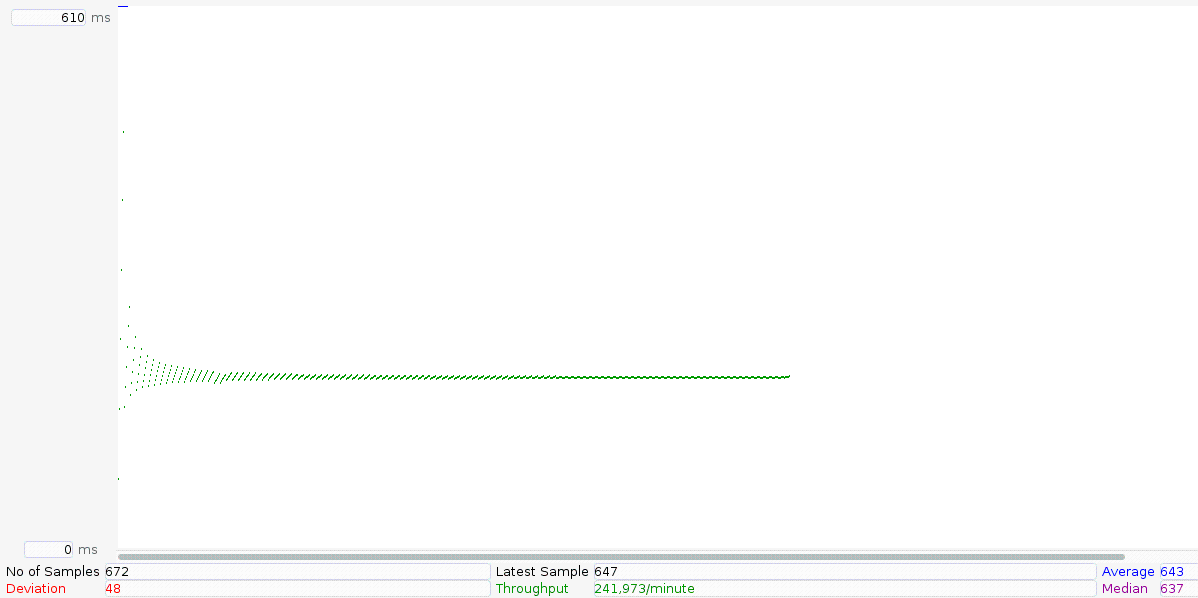
\includegraphics[width=500bp]{img/conf1_graph.png}

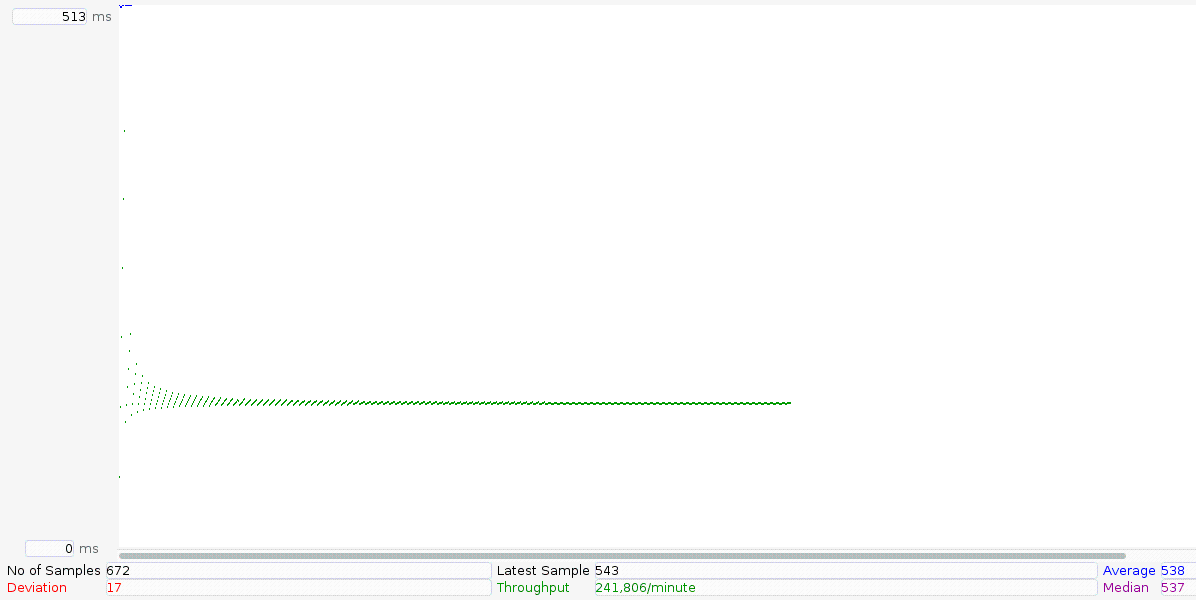
\includegraphics[width=500bp]{img/conf2_graph.png}

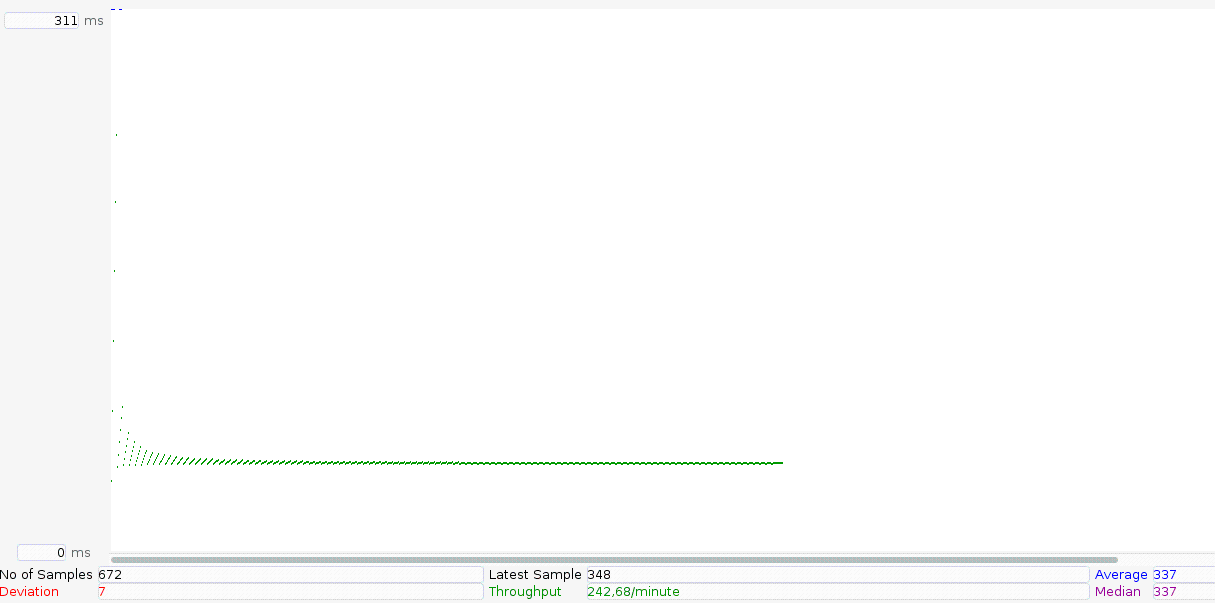
\includegraphics[width=500bp]{img/conf3_graph.png}

Первая конфигурация не удовлетворяет заданным требованиям,

вторая конфигурация справляется с нагрузкой, с небольшим процентом ошибок,

третья конфигурация работает намного быстрее заданного порога, что позволяет

увеличивать нагрузку дальше.

\subsection{Конфигурации для стресс-тестирования}
Для стресс-тестирования для каждой конфигурации постепенно увеличивалась
максимальная пропускная способность до тех пор, пока веб-приложение обрабатывает
запрос в заданные временные рамки.

График строился через элемент Response Time Graph.
\subsection{Графики изменения времени отклика от нагрузки}
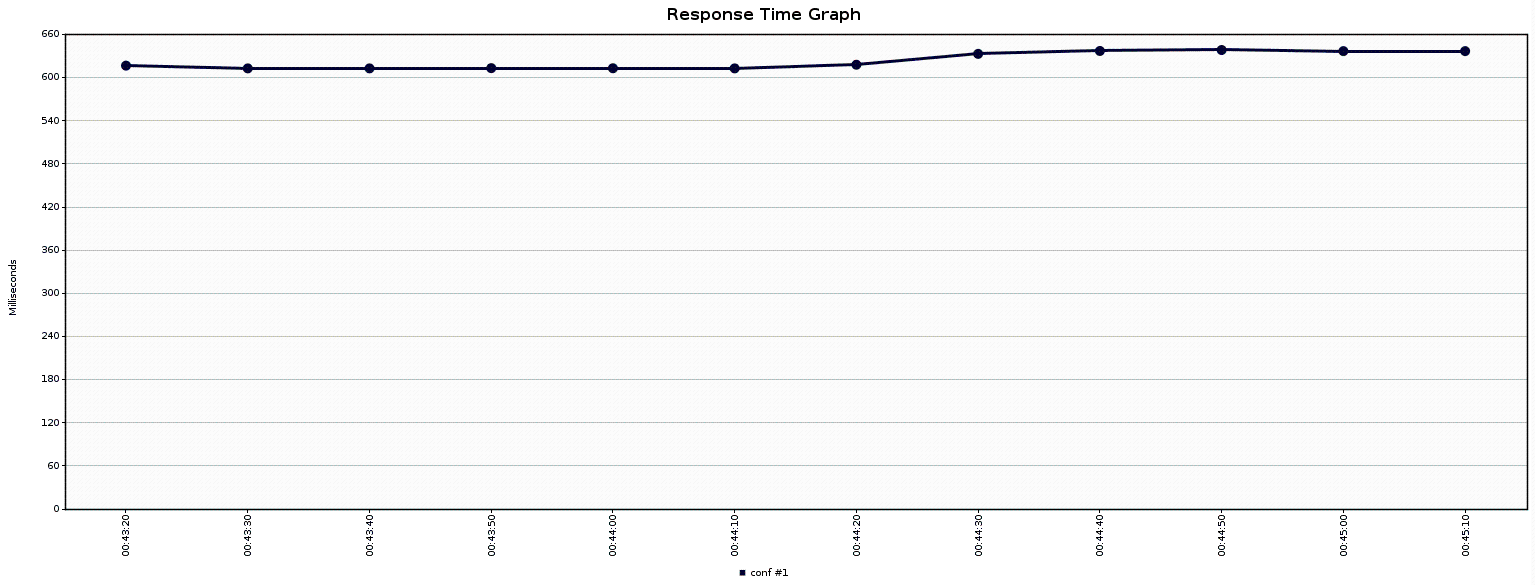
\includegraphics[width=500bp]{img/stress1.png}

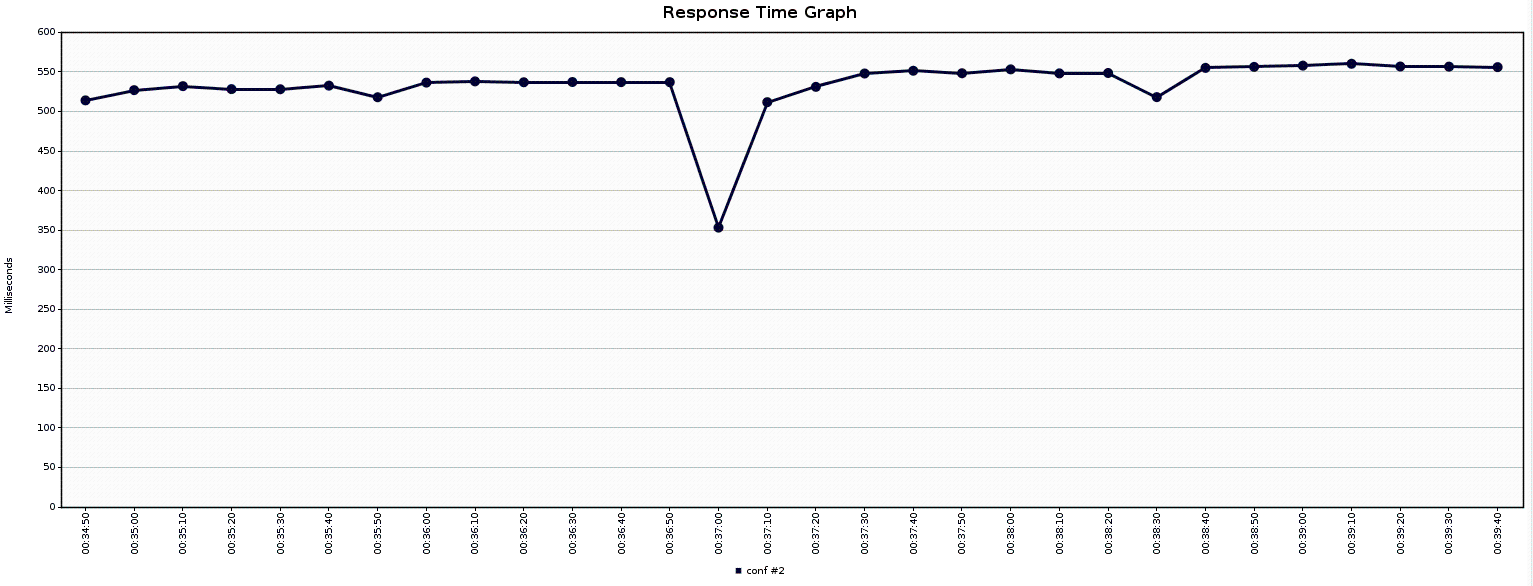
\includegraphics[width=500bp]{img/stress2.png}

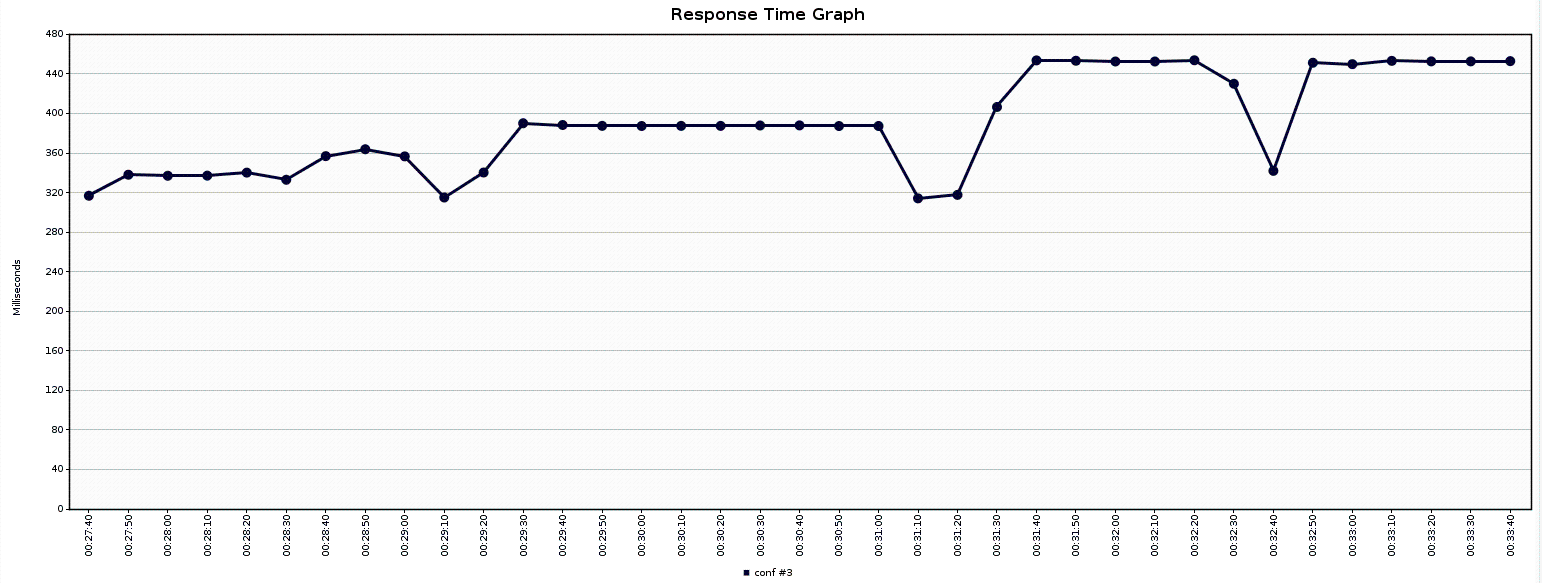
\includegraphics[width=500bp]{img/stress3.png}

Первая конфигурация не удовлетворяет требованиям по времени ответа.

Вторая конфигурация способна выдерживать пропускную способность до 60 запросов
в минуту.

Третья конфигурация справляется с любой нагрузкой при 6 пользователях.

\section{Выводы}

В ходе данной лабораторной работы мы ознакомились с проведением нагрузочного
и стресс-тестирования с помощью Apache Jmeter.

\end{document}
